%%%%%%%%%%%%%%%%%%%%%%%%%%%%%%%%%%%%%%%%%
% a0poster Landscape Poster
% LaTeX Template
% Version 1.0 (22/06/13)
%
% The a0poster class was created by:
% Gerlinde Kettl and Matthias Weiser (tex@kettl.de)
% 
% This template has been downloaded from:
% http://www.LaTeXTemplates.com
%
% License:
% CC BY-NC-SA 3.0 (http://creativecommons.org/licenses/by-nc-sa/3.0/)
%
%%%%%%%%%%%%%%%%%%%%%%%%%%%%%%%%%%%%%%%%%

%----------------------------------------------------------------------------------------
%	PACKAGES AND OTHER DOCUMENT CONFIGURATIONS
%----------------------------------------------------------------------------------------

\documentclass[a0,landscape]{a0poster}

\usepackage{multicol} % This is so we can have multiple columns of text side-by-side
\columnsep=100pt % This is the amount of white space between the columns in the poster
\columnseprule=3pt % This is the thickness of the black line between the columns in the poster

\usepackage[svgnames]{xcolor} % Specify colors by their 'svgnames', for a full list of all colors available see here: http://www.latextemplates.com/svgnames-colors

\usepackage{times} % Use the times font
%\usepackage{palatino} % Uncomment to use the Palatino font

\usepackage{graphicx} % Required for including images
\graphicspath{{figures/}} % Location of the graphics files
\usepackage{booktabs} % Top and bottom rules for table
\usepackage[font=small,labelfont=bf]{caption} % Required for specifying captions to tables and figures
\usepackage{amsfonts, amsmath, amsthm, amssymb} % For math fonts, symbols and environments
\usepackage{wrapfig} % Allows wrapping text around tables and figures
\usepackage{enumitem}
\usepackage{listings}% http://ctan.org/pkg/listings
\usepackage{algorithm}
\usepackage{algpseudocode}
\usepackage{mathtools}
\usepackage{etoolbox}
\AtBeginEnvironment{algorithm}{%
    \setlength{\columnwidth}{\linewidth}%
}
\lstset{
  basicstyle=\ttfamily,
  mathescape
}
\usepackage{pgf,tikz}
\usetikzlibrary{positioning}
\usepackage{pgfplots}
\pgfplotsset{compat=newest}

\DeclareMathOperator{\rank}{rank}
\DeclareMathOperator{\spann}{span}
\newcommand\SPAN[1]{\ensuremath\spann(#1)}

\newtheorem{thm}{Theorem}
\newtheorem{lemma}{Lemma}
%\newtheorem{proposition}{Proposition}
\newtheorem{coro}{Corollary}
%\newtheorem{definition}{Definition}
\newtheorem{remark}{Remark}

\begin{document}

%----------------------------------------------------------------------------------------
%	POSTER HEADER 
%----------------------------------------------------------------------------------------

% The header is divided into three boxes:
% The first is 55% wide and houses the title, subtitle, names and university/organization
% The second is 25% wide and houses contact information
% The third is 19% wide and houses a logo for your university/organization or a photo of you
% The widths of these boxes can be easily edited to accommodate your content as you see fit

\begin{minipage}[b]{0.58\linewidth}
  \veryHuge \color{NavyBlue} \textbf{Automatic Differentiation} \color{Black}\\ % Title
  \Huge\textit{Inside the Black Box at the Heart of Machine Learning}\\[1cm] % Subtitle
  \huge \textbf{Damion A.~Miller}\\ % Author(s)
  \huge Michigan Technological University\\ % University/organization
\end{minipage}
%
\begin{minipage}[b]{0.22\linewidth}
  \Large \textbf{Contact Information:}\\
  Damion A.~Miller\\
  Michigan Technological University\\
  Department of Mathematical Sciences \\
  Houghton, MI\\\\
  Email: \texttt{damionm@mtu.edu}\\ % Email address
\end{minipage}
%
\begin{minipage}[b]{0.19\linewidth}
  \includegraphics[width=20cm]{figures/logo.png} % Logo or a photo of you, adjust its dimensions here\\
  \vspace*{2in}
\end{minipage}

\vspace{1cm} % A bit of extra whitespace between the header and poster content

%----------------------------------------------------------------------------------------

\begin{multicols}{4} % This is how many columns your poster will be broken into, a poster with many figures may benefit from less columns whereas a text-heavy poster benefits from more

%----------------------------------------------------------------------------------------
%	ABSTRACT
%----------------------------------------------------------------------------------------

\begin{abstract}
    Automatic differentiation is a method for accurately and efficiently
    computing derivatives of functions. I implement two different methods, namely,
    forward mode and reverse mode. Furthermore, I explore different combinations
    of these methods for evaluating higher order derivavtives. Using these results we are able to
    apply them to many applications such as machine learning and solving differential
    equations.
\end{abstract}

%----------------------------------------------------------------------------------------

\section*{Motivation}
\begin{itemize}[noitemsep]
\item Derivatives are present in almost all areas of engineering.
\item Relevant in machine learning where the gradient (a derivative
    in the direction of steepest ascent) must be calulated repeatedly
    over functions with a large number of inputs.
\end{itemize}
\section*{Computational Graph}
    Let $f:\mathbb{R}^n\rightarrow\mathbb{R}$ and $\vec{x}=(x_1,x_2,\dots,x_n)^T\in\mathbb{R}^n$

    Then one of four cases (Binary, Unary, Trivial, Constant):
\begin{align*}
    1.\ f(\vec{x})&=g(\vec{x})\odot h(\vec{x}) &&\odot\in\{+,-,*,/,\dots\} \\
    2.\ f(\vec{x})&=g(h(\vec{x})) &&g(x)\in\{\cos{(x)},\sin{(x)},\exp{(x)},\log{(x)},\dots\} \\
    3.\ f(\vec{x})&=x_i &&1\leq i\leq n \\
    4.\ f(\vec{x})&=\alpha &&\alpha\in\mathbb{R}
\end{align*}

We can build a computational graph of $f(\vec{x})$ by recursing on $h(\vec{x})$ (and $g(\vec{x})$ in case 1) until case 3 or 4 are returned.

\subsubsection*{Example: $f(x_1,x_2)=x_1*x_2+\sin{(x_1)}$}

\begin{center}
\begin{tikzpicture}[main/.style = {draw, circle, minimum size = 2cm}]
    \node[main] (1) [label={180:$w_1$}]{$x_1$};
    \node[main] (2) [right = 1cm of 1][label={0:$w_2$}] {$x_2$};
    \node[main] (3) [above = 1cm of 1][label={180:$\sin{(w_1)}=w_3$}] {$\sin$};
    \node[main] (4) [above = 1cm of 2][label={0:$w_4=w_1*w_2$}] {$*$};
    \node[main] (5) [above = 1cm of 3][label={0:$w_5=w_3+w_4$}]{$+$};
    \draw (1) -- (3);
    \draw (1) -- (4);
    \draw (2) -- (4);
    \draw (3) -- (5);
    \draw (4) -- (5);
\end{tikzpicture}
\end{center}

\section*{Forward Mode}
Case 1: Binary (product rule, quotient rule, etc.) 

    Given $\left(g(\vec{x}),\frac{\partial g}{\partial\vec{z}}\right),\left(h(\vec{x}),\frac{\partial h}{\partial\vec{z}}\right)$, and $f(\vec{x})=g(\vec{x})\odot h(\vec{x})$
    \begin{equation}
        \frac{\partial f}{\partial\vec{z}}=
            \begin{cases}
                \frac{\partial g}{\partial\vec{z}}\pm\frac{\partial h}{\partial\vec{z}} & \text{if } \odot = \pm\\
                g(\vec{x})\frac{\partial h}{\partial\vec{z}} + h(\vec{x})\frac{\partial g}{\partial\vec{z}} & \text{if } \odot = *\\
                \frac{h(\vec{x})\frac{\partial g}{\partial\vec{z}} - g(\vec{x})\frac{\partial h}{\partial\vec{z}}}{(h(\vec{x}))^2} & \text{if } \odot = /\\
                \dots
            \end{cases}
    \end{equation}

\vspace{10cm}
Case 2: Unary (chain rule)

    Given $\left(h(\vec{x}),\frac{\partial h}{\partial\vec{z}}\right)$ and $f(\vec{x})=g(h(\vec{x}))$
    \begin{equation}
        \frac{\partial f}{\partial\vec{z}}=\frac{\partial}{\partial\vec{z}}\;g(h(\vec{x}))=\underbracket{\frac{dg}{dh}}_{\text{trivial}}*\underbracket{\frac{\partial h}{\partial\vec{z}}}_{\text{given}}
    \end{equation}
    \begin{equation}
        \frac{dg}{dh}=
            \begin{cases}
                \cos{(h(\vec{x}))} & \text{if } g(x) = \sin{(x)}\\
                \exp{(h(\vec{x}))} & \text{if } g(x) = \exp{(x)}\\
                \frac{1}{h(\vec{x})} & \text{if } g(x) = \log{(x)}\\
                \dots
            \end{cases}
    \end{equation}
Case 3:
    
\begin{thm}
    Let $f(\vec{x})$ be the function $f(\vec{x})=x_i$ where $\vec{x}=(x_1,x_2,\dots,x_n)^T$ and $1\leq i\leq n$.
    Let $\vec{z}\in\mathbb{R}^n$ be a unit vector. 
    Then $\frac{\partial}{\partial\vec{z}}f(\vec{x})=z_i$.
    \begin{proof}
        $$\frac{\partial}{\partial\vec{z}}f(\vec{x})=\lim_{h\rightarrow0}\frac{f(\vec{x} + h\vec{z}) - f(\vec{x})}{h}=\lim_{h\rightarrow0}\frac{x_i + hz_i - x_i}{h}=z_i.$$
    \end{proof}
\end{thm}
\subsection*{Dual Numbers}
A dual number of a fuction $f(\vec{x})$ is defined to be the tuple: 
$$\left(f(\vec{x}),\frac{\partial}{\partial\vec{z}}\;f(\vec{x})\right).$$

\subsection*{Implementation}
\begin{center}
    \includegraphics[width=250mm]{figures/forward_mode.png}
\end{center}
\begin{algorithm}[H]
\caption{Forward Mode}
    \hspace*{\algorithmicindent} \textbf{Input}: $f(\vec{x}),\vec{x},\vec{z}$ \\
    \hspace*{\algorithmicindent} \textbf{Output}: Dual$\left(f(\vec{x}),\frac{\partial}{\partial\vec{z}}f(\vec{x})\right)$
\begin{algorithmic}[1]
\State initialize vector $D$ of $n$ dual numbers
    \For{$i\gets 1\textbf{ to }n$}
        \State $D_i\gets Dual(x_i, z_i)$
    \EndFor\\
\Return $f(D)$
\end{algorithmic}
\end{algorithm}

\section*{Reverse Mode}

\subsection*{Adjoint}
The adjoint of some intermediate function $w_i=g(\vec{x})$ in a computational graph of $f(\vec{x})$ is defined to be:
$$\dot{w_i}=\frac{\partial f}{\partial w_i}$$

\subsubsection*{Key Observations}
\begin{itemize}
\item Let $P$ be the set of parents of some intermediate function $w_i$, then
    \begin{equation}
\dot{w_i}=\frac{\partial f}{\partial w_i}=\sum_{w_j\in P}{\frac{\partial f}{\partial w_j}\frac{\partial w_j}{\partial w_i}}
    \end{equation}
\item The final node in our compuation graph has an adjoint of 1.
\item Each node $w_i$ has at most 2 children which have adjoint's dependent on $\dot{w_i}$.
\item Our base case is at the end instead of the beginning of the function evaluation.
\end{itemize}

\subsection*{Implementation}
\subsubsection*{Tape}
We use a tape to record the computational graph of our function. Using an array for
the tape will help reduce memory access time. 

\vspace{5mm}
\begin{center}
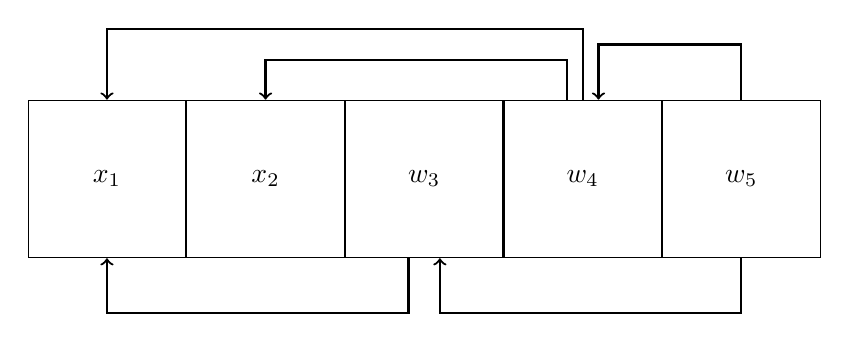
\begin{tikzpicture}[main/.style = {draw, minimum size = 2cm}]
    \node[main] (1) {$x_1$};
    \node[main] (2) [right = 0mm of 1] {$x_2$};
    \node[main] (3) [right = 0mm of 2] {$w_3$};
    \node[main] (4) [right = 0mm of 3] {$w_4$};
    \node[main] (5) [right = 0mm of 4] {$w_5$};
    \path[draw, thick, <-]
        (1.south) -- ++ (0,-7mm) to 
        ([yshift=-7mm] 2.south) -| ([xshift=-2mm] 3.south) -- (3);
    \path[draw, thick, <-]
        ([xshift=2mm]3.south) -- ++ (0,-7mm) to 
        ([yshift=-7mm] 4.south) -| ([xshift=0mm] 5.south) -- (5);
    \path[draw, thick, <-]
        ([xshift=2mm]4.north) -- ++ (0,7mm) to 
        ([yshift=7mm] 5.north) -| ([xshift=0mm] 5.north) -- (5);
    \path[draw, thick, <-]
        (2.north) -- ++ (0,5mm) to 
        ([yshift=5mm] 3.north) -| ([xshift=-2mm] 4.north) -- (4);
    \path[draw, thick, <-]
        (1.north) -- ++ (0,9mm) to 
        ([yshift=9mm] 2.north) -| ([xshift=0mm] 4.north) -- (4);
\end{tikzpicture}
\end{center}

\subsubsection*{Node}
Each element of our tape is a node in our computational graph that stores the following:
\begin{itemize}
    \item The value of the function evaluated at a given point.
    \item The adjoint of the function.
    \item The indices of itself and (up to) two children.
    \item The trivial derivatives with repsect to the children.
    \item A reference to the tape itself.
\end{itemize}

\subsubsection*{Operator Overloading}
Similar to forward mode, we will use operator overloading to build our tape, that
is whenever an operation is called on two nodes, we wish to add a new node
representing its composition function to the end of our tape.

\begin{algorithm}[H]
\caption{Reverse Mode}
    \hspace*{\algorithmicindent} \textbf{Input}: $f(\vec{x}),\vec{x}$ \\
    \hspace*{\algorithmicindent} \textbf{Output}: $\nabla f(\vec{x})$
\begin{algorithmic}[1]
\State $c\gets$ number of nodes in computational graph
\State initialize array $tape$ of $c$ Nodes
\For{$i\gets 1\textbf{ to }n$}
    \State $tape[i]\gets Node(x_i, 0, [i,0,0], [0,0], tape)$
\EndFor\\
$f(tape[1\dots n])$ 
    \State $tape[c].adjoint\gets 1$
\For{$i\gets c\textbf{ down to }n+1$}
    \State $tape[child1]+=tape[i].adjoint*tape[i].derivative1$
    \State $tape[child2]+=tape[i].adjoint*tape[i].derivative2$
\EndFor\\
    \Return $tape[1\dots n].adjoint$
\end{algorithmic}
\end{algorithm}

\section*{Results}
\subsection*{Gradient}
\begin{center}
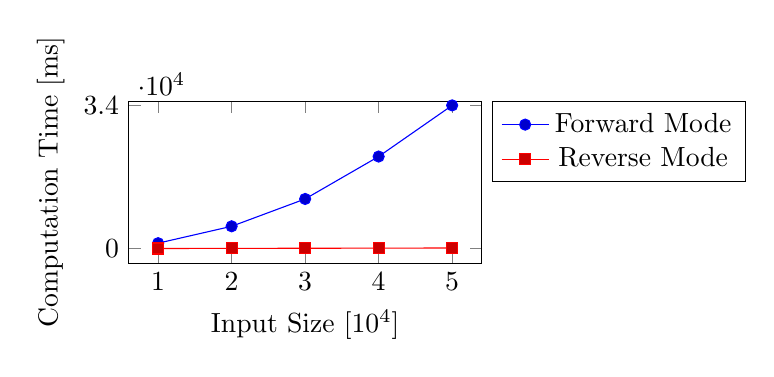
\begin{tikzpicture}
\begin{axis}[
        xlabel={Input Size [$10^4$]},
xtick={0,1,2,3,4,5},
ytick={0,34000},
ymax = 35000,
legend pos = outer north east,
    ylabel={Computation Time [ms]},
width=0.5\linewidth,
height=0.3\linewidth
]

\addplot coordinates {
    (1,1289.206)
    (2,5298.345)
    (3,11796.312)
    (4,21877.891)
    (5,34033.270)
};
\addlegendentry{Forward Mode}

\addplot coordinates {
    (1,025.315)
    (2,050.880)
    (3,0081.533)
    (4,0109.979)
    (5,0141.833)
};
\addlegendentry{Reverse Mode}

\end{axis}
\end{tikzpicture}
    \captionof{figure}{A plot comparing the computation time of reverse and forward
    mode calculating the gradient of various instances of the Rosenbrock function. The key observation
    here is that forward mode grows proportional to $n^2$ compared to only $n$ for reverse.}
\end{center}

\subsection*{Hessian}
We may calculate higher order derivatives by performing multiple instances of reverse and/or
forward mode. From these higher order derivatives we can form structures such as the Hessian matrix.

\begin{center}
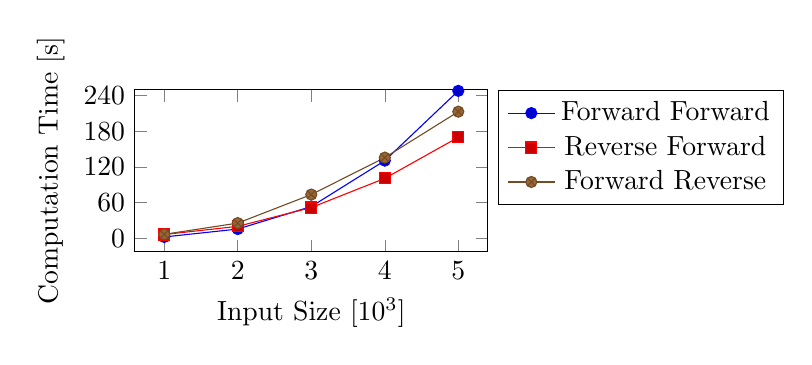
\begin{tikzpicture}
\begin{axis}[
        xlabel={Input Size [$10^3$]},
xtick={0,1,2,3,4,5},
ytick={0, 60, 120, 180, 240},
ymax = 250,
legend pos = outer north east,
    ylabel={Computation Time [s]},
width=0.5\linewidth,
height=0.3\linewidth
]

\addplot coordinates {
    (1,1.93897)
    (2,15.271401)
    (3,53.221918)
    (4,130.57251)
    (5,248.190596)
};
\addlegendentry{Forward Forward}

\addplot coordinates {
    (1,6.073335)
    (2,19.824306)
    (3,51.5246)
    (4,100.625566)
    (5,169.947057)
};
\addlegendentry{Reverse Forward}

\addplot coordinates {
    (1,6.416108)
    (2,25.326868)
    (3,73.401066)
    (4,135.731482)
    (5,213.101433)
};
\addlegendentry{Forward Reverse}

\end{axis}
\end{tikzpicture}
    \captionof{figure}{A plot comparing the computation time of the Hessian matrix
    on the Rosenbrock function using different combinations of automatic differentiation.}
\end{center}

\section*{Future Work}
\begin{itemize}
    \item Continue research here at Michigan Tech for the remainder of the semester under the supervision of B. W. Ong.
    \item Improve the efficiency of higher order derivative implementations.
    \item Minimize the space used for each Node in reverse mode.
    \item Construct reusable tape for faster sequential reverse passes.
\end{itemize}

\section*{References}
\begin{enumerate}[{label=[\arabic{*}]}]
    \item Revels, Jarrett, Miles Lubin, and Theodore Papamarkou. "Forward-mode automatic differentiation in Julia." arXiv preprint arXiv:1607.07892 (2016).
    \item Tom J. Smeding and Matthijs I. L. Vákár. 2023. Efficient Dual-Numbers Reverse AD via Well-Known Program Transformations. Proc. ACM Program. Lang. 7, POPL, Article 54 (January 2023), 28 pages. https://doi.org/10.1145/3571247
\end{enumerate}

\end{multicols}
\end{document}
